% Chapter: 06_edinburgh
% Standalone talk: Intro to Neural Networks & Mechanistic Interpretability
% Edinburgh seminar "Maths, Physics, and AI Alignment", 11 May 2026

% ============================================================
% Overview
% ============================================================

\begin{frame}{Overview}
\begin{enumerate}
\item \textbf{Machine Learning}
  \begin{enumerate}
  \item[1.1] Concepts
  \item[1.2] Architectures
  \end{enumerate}
\item \textbf{Mechanistic Interpretability}
\item \textbf{Features}
\item \textbf{Circuits}
\item \textbf{Open Problems}
\end{enumerate}
\end{frame}

% ============================================================
% Chapter navigation command
% ============================================================

% ============================================================
\section{Machine Learning}
% ============================================================

% ------------------------------------------------------------
\subsection{Concepts}
% ------------------------------------------------------------

\begin{frame}{}
\begin{enumerate}
\item \textbf{\large Machine Learning}
  \begin{enumerate}
  \item[1.1] \textbf{Concepts} $\leftarrow$
  \item[1.2] \textcolor{gray}{Architectures}
  \end{enumerate}
\item \textcolor{gray}{Mechanistic Interpretability}
\item \textcolor{gray}{Features}
\item \textcolor{gray}{Circuits}
\item \textcolor{gray}{Open Problems}
\end{enumerate}
\end{frame}

\begin{frame}{The Training Loop}
\begin{center}
\begin{tikzpicture}[
  box/.style={rectangle, draw, thick, rounded corners=3pt, minimum width=2.2cm, minimum height=1.8cm, font=\small, align=center},
  arr/.style={->, very thick, gray!70},
]
  % Boxes
  \node[box, fill=blue!15] (data) at (0, 0) {
    \textbf{Data}\\[0.3em]
    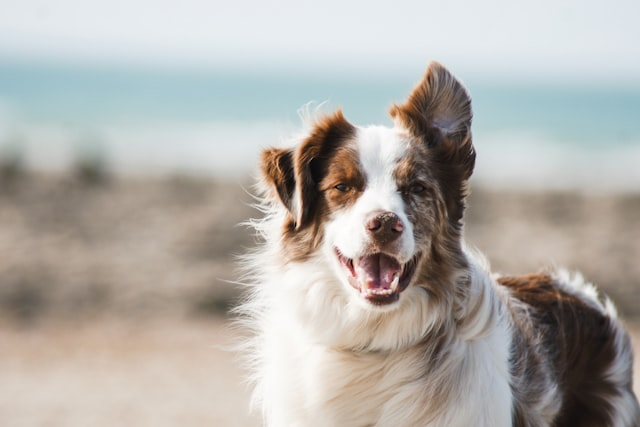
\includegraphics[width=1.4cm]{figures/dog.jpg}
  };
  \node[box, fill=green!15] (model) at (3.8, 0) {
    \textbf{Model}\\[0.3em]
    {\tiny\begin{tikzpicture}[scale=0.25,
      n/.style={circle, draw, thick, fill=orange!20, minimum size=2mm, inner sep=0pt}]
      \foreach \i in {1,2,3} { \node[n] (i\i) at (0, -\i*0.8) {}; }
      \foreach \j in {1,2} { \node[n] (h\j) at (1.5, -\j*0.8-0.4) {}; }
      \node[n] (o1) at (3, -1.6) {};
      \foreach \i in {1,2,3} \foreach \j in {1,2} \draw[gray, thin] (i\i) -- (h\j);
      \foreach \j in {1,2} \draw[gray, thin] (h\j) -- (o1);
    \end{tikzpicture}}
  };
  \node[box, fill=red!15] (pred) at (7.6, 0) {
    \textbf{Prediction}\\[0.3em]
    {\scriptsize cat: 30\%}\\
    {\scriptsize\textbf{dog: 70\%}}
  };
  \node[box, fill=yellow!15, minimum width=2.2cm] (loss) at (11.4, 0) {
    \textbf{Loss}\\[0.3em]
    {\scriptsize $-\log(0.7)$}
  };
  \node[box, fill=orange!15, minimum width=2.8cm] (opt) at (5.7, -3.2) {
    \textbf{Optimizer}\\[0.3em]
    {\scriptsize $\theta \leftarrow \theta - \alpha \nabla_\theta \mathcal{L}$}
  };

  % Arrows
  \draw[arr] (data) -- (model);
  \draw[arr] (model) -- (pred);
  \draw[arr] (pred) -- (loss);
  \draw[arr] (loss) |- (opt);
  \draw[arr] (opt) -| (model);
\end{tikzpicture}
\end{center}
\end{frame}

\begin{frame}{Forward Pass / Backward Pass}
\begin{center}
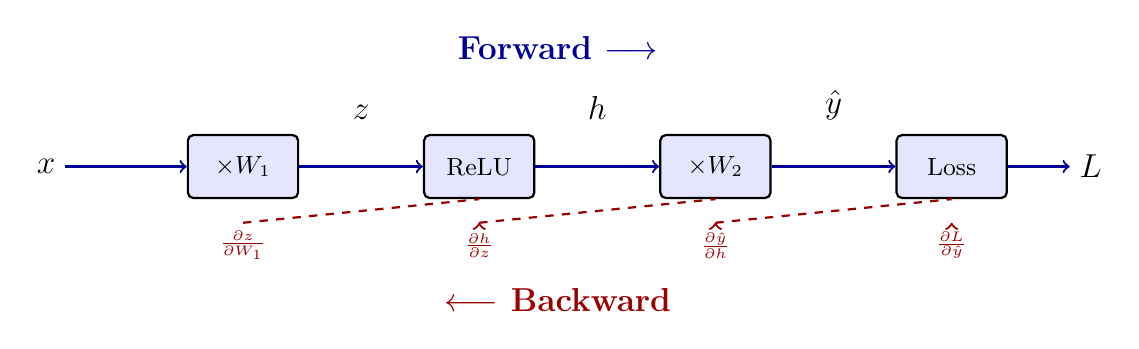
\begin{tikzpicture}[
  op/.style={rectangle, draw, thick, rounded corners=2pt, minimum width=1.4cm, minimum height=0.8cm, font=\small},
  val/.style={font=\large},
  farr/.style={->, thick, blue!60!black},
  barr/.style={<-, thick, red!60!black, dashed},
]
  % Forward pass nodes
  \node[val] (x) at (0, 0) {$x$};
  \node[op, fill=blue!10] (mul1) at (2.5, 0) {$\times W_1$};
  \node[op, fill=blue!10] (relu) at (5.5, 0) {ReLU};
  \node[op, fill=blue!10] (mul2) at (8.5, 0) {$\times W_2$};
  \node[op, fill=blue!10] (lossn) at (11.5, 0) {Loss};
  \node[val, right] at (13, 0) {$L$};

  % Intermediate labels
  \node[val, above=2pt] at (4, 0.4) {$z$};
  \node[val, above=2pt] at (7, 0.4) {$h$};
  \node[val, above=2pt] at (10, 0.4) {$\hat{y}$};

  % Forward arrows
  \draw[farr] (x) -- (mul1);
  \draw[farr] (mul1) -- (relu);
  \draw[farr] (relu) -- (mul2);
  \draw[farr] (mul2) -- (lossn);
  \draw[farr] (lossn) -- (13, 0);

  % Labels
  \node[blue!60!black, font=\large\bfseries] at (6.5, 1.5) {Forward $\longrightarrow$};
  \node[red!60!black, font=\large\bfseries] at (6.5, -1.7) {$\longleftarrow$ Backward};

  % Backward arrows
  \draw[barr] (mul1.south) ++(0,-0.3) -- (relu.south) ++(0,-0.3);
  \draw[barr] (relu.south) ++(0,-0.3) -- (mul2.south) ++(0,-0.3);
  \draw[barr] (mul2.south) ++(0,-0.3) -- (lossn.south) ++(0,-0.3);

  % Gradient labels below backward arrows
  \node[val, red!60!black] at (2.5, -1) {\scriptsize $\frac{\partial z}{\partial W_1}$};
  \node[val, red!60!black] at (5.5, -1) {\scriptsize $\frac{\partial h}{\partial z}$};
  \node[val, red!60!black] at (8.5, -1) {\scriptsize $\frac{\partial \hat{y}}{\partial h}$};
  \node[val, red!60!black] at (11.5, -1) {\scriptsize $\frac{\partial L}{\partial \hat{y}}$};
\end{tikzpicture}
\end{center}

\vspace{0.5em}
\textbf{Chain rule:}
\[
\frac{\partial L}{\partial W_1}
= \textcolor{red!60!black}{\frac{\partial L}{\partial \hat{y}}}
\cdot \textcolor{red!60!black}{\frac{\partial \hat{y}}{\partial h}}
\cdot \textcolor{red!60!black}{\frac{\partial h}{\partial z}}
\cdot \textcolor{red!60!black}{\frac{\partial z}{\partial W_1}}
\]
\end{frame}

\begin{frame}{Train Loss vs.\ Test Loss}
\begin{center}
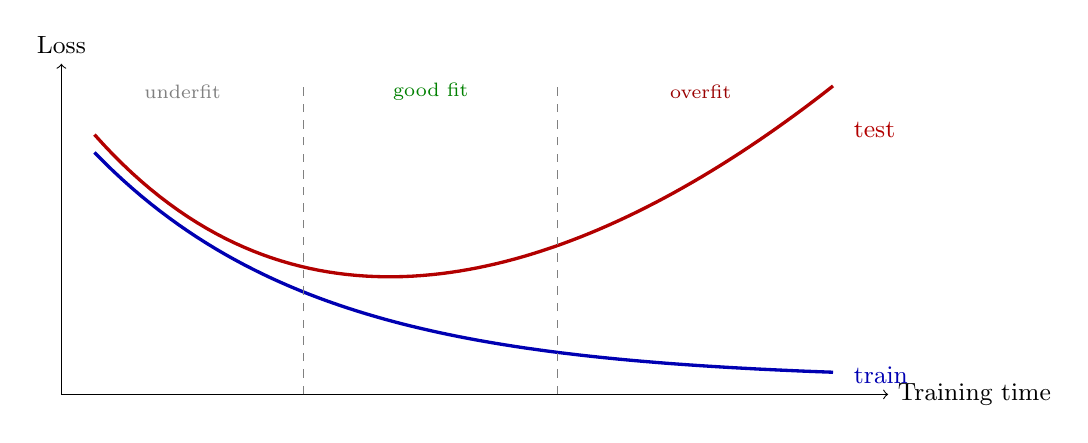
\begin{tikzpicture}[xscale=1.4, yscale=1.2]
  \draw[->] (0, 0) -- (7.5, 0) node[right, font=\small] {Training time};
  \draw[->] (0, 0) -- (0, 3.5) node[above, font=\small] {Loss};

  % Train loss (always decreasing)
  \draw[very thick, blue!70!black, domain=0.3:7, samples=80]
    plot (\x, {2.8*exp(-0.5*\x) + 0.15});
  \node[blue!70!black, font=\small, right] at (7.1, 0.2) {train};

  % Test loss (U-shaped)
  \draw[very thick, red!70!black, domain=0.3:7, samples=80]
    plot (\x, {2.8*exp(-0.5*\x) + 0.08*(\x-1)*(\x-1) + 0.3});
  \node[red!70!black, font=\small, right] at (7.1, 2.8) {test};

  % Regions
  \draw[dashed, gray] (2.2, 0) -- (2.2, 3.3);
  \draw[dashed, gray] (4.5, 0) -- (4.5, 3.3);

  \node[font=\scriptsize, gray, align=center] at (1.1, 3.2) {underfit};
  \node[font=\scriptsize, green!50!black, align=center] at (3.35, 3.2) {good fit};
  \node[font=\scriptsize, red!60!black, align=center] at (5.8, 3.2) {overfit};
\end{tikzpicture}
\end{center}
\end{frame}

\begin{frame}{Double Descent}
\begin{center}
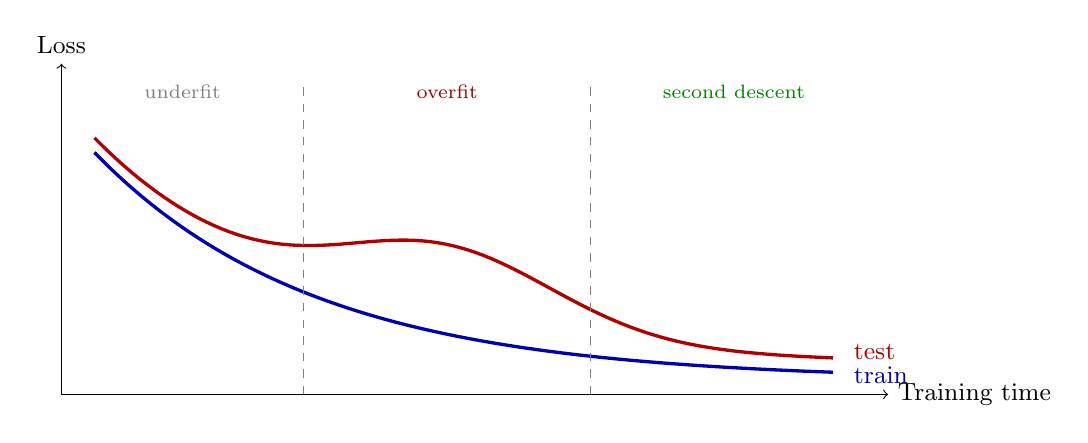
\begin{tikzpicture}[xscale=1.4, yscale=1.2]
  \draw[->] (0, 0) -- (7.5, 0) node[right, font=\small] {Training time};
  \draw[->] (0, 0) -- (0, 3.5) node[above, font=\small] {Loss};

  % Train loss (always decreasing)
  \draw[very thick, blue!70!black, domain=0.3:7, samples=80]
    plot (\x, {2.8*exp(-0.5*\x) + 0.15});
  \node[blue!70!black, font=\small, right] at (7.1, 0.2) {train};

  % Test loss (U then down again)
  \draw[very thick, red!70!black, domain=0.3:7, samples=100]
    plot (\x, {2.8*exp(-0.5*\x) + 0.8*exp(-0.5*(\x-3.5)*(\x-3.5)) + 0.3});
  \node[red!70!black, font=\small, right] at (7.1, 0.45) {test};

  % Regions
  \draw[dashed, gray] (2.2, 0) -- (2.2, 3.3);
  \draw[dashed, gray] (4.8, 0) -- (4.8, 3.3);

  \node[font=\scriptsize, gray, align=center] at (1.1, 3.2) {underfit};
  \node[font=\scriptsize, red!60!black, align=center] at (3.5, 3.2) {overfit};
  \node[font=\scriptsize, green!50!black, align=center] at (6.1, 3.2) {second descent};
\end{tikzpicture}
\end{center}

\source{nakkiran2019}
\end{frame}

\begin{frame}{Grokking}
\begin{center}
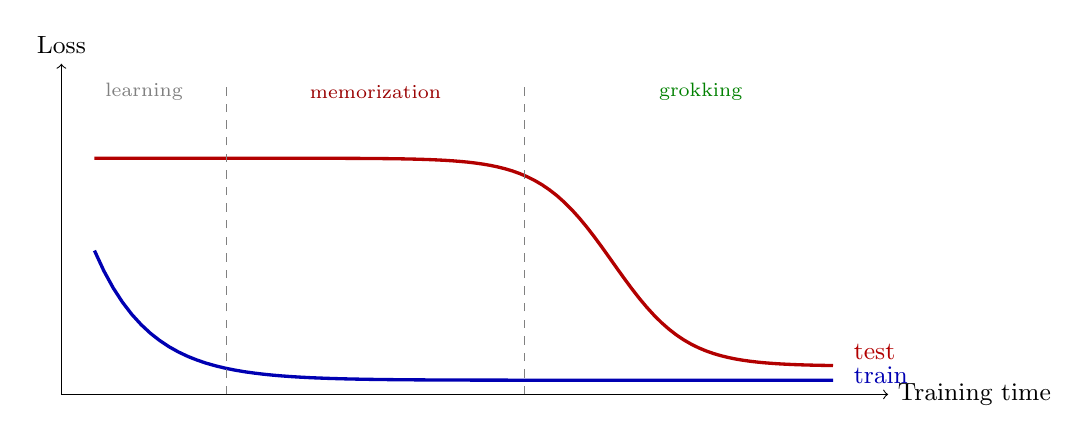
\begin{tikzpicture}[xscale=1.4, yscale=1.2]
  \draw[->] (0, 0) -- (7.5, 0) node[right, font=\small] {Training time};
  \draw[->] (0, 0) -- (0, 3.5) node[above, font=\small] {Loss};

  % Train loss (drops quickly)
  \draw[very thick, blue!70!black, domain=0.3:7, samples=80]
    plot (\x, {2.5*exp(-2*\x) + 0.15});
  \node[blue!70!black, font=\small, right] at (7.1, 0.2) {train};

  % Test loss (stays high, then suddenly drops)
  \draw[very thick, red!70!black, domain=0.3:7, samples=100]
    plot (\x, {2.2/(1 + exp(3*(\x-5))) + 0.3});
  \node[red!70!black, font=\small, right] at (7.1, 0.45) {test};

  % Regions
  \draw[dashed, gray] (1.5, 0) -- (1.5, 3.3);
  \draw[dashed, gray] (4.2, 0) -- (4.2, 3.3);

  \node[font=\scriptsize, gray, align=center] at (0.75, 3.2) {learning};
  \node[font=\scriptsize, red!60!black, align=center] at (2.85, 3.2) {memorization};
  \node[font=\scriptsize, green!50!black, align=center] at (5.8, 3.2) {grokking};
\end{tikzpicture}
\end{center}

\source{power2022}
\end{frame}

\begin{frame}{Definitions}
\begin{description}
\item[Parameter / Weight] the numbers that define the model, updated during training ($\theta$, $W$, $b$)
\item[Activation] intermediate values computed during a forward pass
\item[Hyperparameter] choices made \emph{before} training: learning rate, architecture, batch size
\end{description}
\end{frame}

% ------------------------------------------------------------
\subsection{Architectures}
% ------------------------------------------------------------

\begin{frame}{}
\begin{enumerate}
\item \textbf{\large Machine Learning}
  \begin{enumerate}
  \item[1.1] Concepts
  \item[1.2] \textbf{Architectures} $\leftarrow$
  \end{enumerate}
\item \textcolor{gray}{Mechanistic Interpretability}
\item \textcolor{gray}{Features}
\item \textcolor{gray}{Circuits}
\item \textcolor{gray}{Open Problems}
\end{enumerate}
\end{frame}

\begin{frame}{Multi-Layer Perceptron}
\begin{columns}[c]
\begin{column}{0.55\textwidth}
\begin{center}
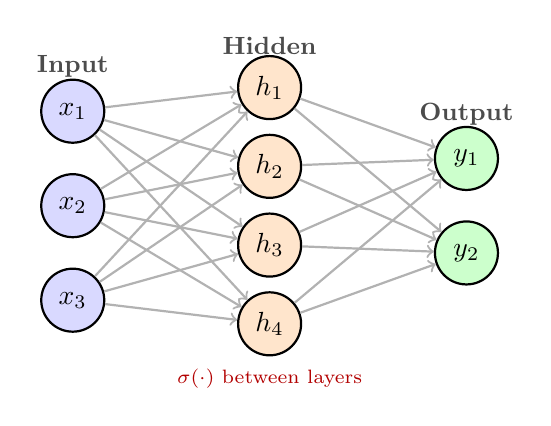
\begin{tikzpicture}[
  neuron/.style={circle, draw, thick, minimum size=8mm, inner sep=0pt},
  input/.style={neuron, fill=blue!15},
  hidden/.style={neuron, fill=orange!20},
  output/.style={neuron, fill=green!20},
  conn/.style={->, thick, gray!60},
  annot/.style={font=\small\bfseries, text=black!70},
]
  \foreach \i in {1,2,3} {
    \node[input] (i\i) at (0, -\i*1.2+2.4) {$x_{\i}$};
  }
  \foreach \j in {1,2,3,4} {
    \node[hidden] (h\j) at (2.5, -\j*1.0+2.5) {$h_{\j}$};
  }
  \foreach \k in {1,2} {
    \node[output] (o\k) at (5, -\k*1.2+1.8) {$y_{\k}$};
  }
  \foreach \i in {1,2,3}
    \foreach \j in {1,2,3,4}
      \draw[conn] (i\i) -- (h\j);
  \foreach \j in {1,2,3,4}
    \foreach \k in {1,2}
      \draw[conn] (h\j) -- (o\k);
  \node[annot, above=3mm] at (0, 1.2) {Input};
  \node[annot, above=3mm] at (2.5, 1.5) {Hidden};
  \node[annot, above=3mm] at (5, 0.6) {Output};

  % nonlinearity label
  \node[font=\scriptsize, red!70!black] at (2.5, -2.2) {$\sigma(\cdot)$ between layers};
\end{tikzpicture}
\end{center}
\end{column}
\begin{column}{0.42\textwidth}
$$h = \sigma(W_1 x + b_1)$$
$$y = W_2 h + b_2$$

\vspace{1em}
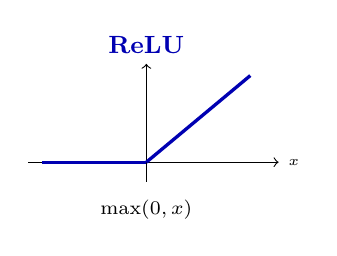
\begin{tikzpicture}[xscale=0.6, yscale=0.5]
  \draw[->] (-2.5, 0) -- (2.8, 0) node[right, font=\tiny] {$x$};
  \draw[->] (0, -0.5) -- (0, 2.5);
  \draw[very thick, blue!70!black] (-2.2, 0) -- (0, 0);
  \draw[very thick, blue!70!black] (0, 0) -- (2.2, 2.2);
  \node[above, font=\small\bfseries, blue!70!black] at (0, 2.5) {ReLU};
  \node[below, font=\scriptsize] at (0, -0.7) {$\max(0, x)$};
\end{tikzpicture}
\end{column}
\end{columns}
\end{frame}

\begin{frame}{Universal Approximation Theorem}
\vfill
A neural network with a single hidden layer and a nonlinear activation function
can approximate any continuous function on a compact set to arbitrary precision,
given enough neurons.
\vfill

\source{cybenko1989}
\end{frame}

\begin{frame}{Universal Approximation: Intuition}
\begin{center}
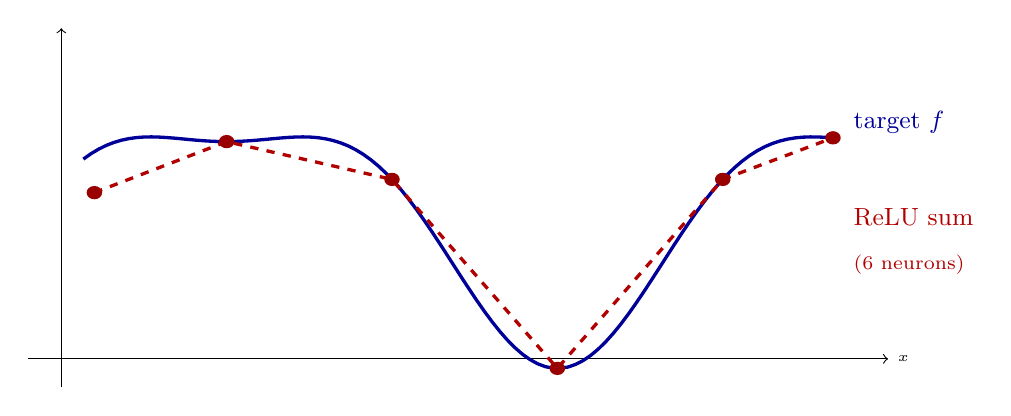
\begin{tikzpicture}[xscale=1.4, yscale=1.2]
  \draw[->] (-0.3, 0) -- (7.5, 0) node[right, font=\tiny] {$x$};
  \draw[->] (0, -0.3) -- (0, 3.5);
  \draw[very thick, blue!60!black, domain=0.2:7, samples=100]
    plot (\x, {1.5 + 1.2*sin(\x*60) + 0.4*cos(\x*120)});
  \node[blue!60!black, font=\small, right] at (7.1, 2.5) {target $f$};
  \draw[very thick, red!70!black, dashed]
    (0.3, 1.76) -- (1.5, 2.30) -- (3.0, 1.90) -- (4.5, -0.10) --
    (6.0, 1.90) -- (7.0, 2.34);
  \node[red!70!black, font=\small, right] at (7.1, 1.5) {ReLU sum};
  \node[red!70!black, font=\scriptsize, right] at (7.1, 1.0) {(6 neurons)};
  \foreach \px/\py in {0.3/1.76, 1.5/2.30, 3.0/1.90, 4.5/-0.10, 6.0/1.90, 7.0/2.34} {
    \fill[red!60!black] (\px, \py) circle (2pt);
  }
\end{tikzpicture}
\end{center}
\end{frame}

\begin{frame}{Layers}
\begin{center}
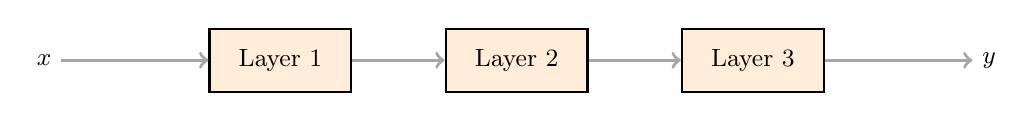
\begin{tikzpicture}[
  box/.style={rectangle, draw, thick, fill=orange!15, minimum width=1.8cm, minimum height=0.8cm, font=\small},
  arr/.style={->, very thick, gray!70},
]
  \node[font=\small] (inp) at (0, 0) {$x$};
  \node[box] (l1) at (3, 0) {Layer 1};
  \node[box] (l2) at (6, 0) {Layer 2};
  \node[box] (l3) at (9, 0) {Layer 3};
  \node[font=\small] (out) at (12, 0) {$y$};

  \draw[arr] (inp) -- (l1);
  \draw[arr] (l1) -- (l2);
  \draw[arr] (l2) -- (l3);
  \draw[arr] (l3) -- (out);
\end{tikzpicture}
\end{center}
\end{frame}

\begin{frame}{Residual Connections}
% Top: fork-and-merge with explicit fork dots
\begin{center}
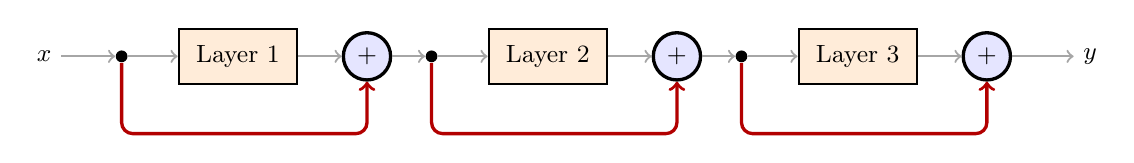
\begin{tikzpicture}[
  box/.style={rectangle, draw, thick, fill=orange!15, minimum width=1.5cm, minimum height=0.7cm, font=\small},
  arr/.style={->, thick, gray!70},
  plus/.style={circle, draw, very thick, fill=blue!10, minimum size=6mm, inner sep=0pt, font=\small\bfseries},
  dot/.style={circle, fill=black, inner sep=1.5pt},
  xscale=0.82,
]
  % Fork points, layers, sum nodes
  \node[font=\small] (inp) at (0, 0) {$x$};
  \node[dot] (d1) at (1.2, 0) {};
  \node[box] (l1) at (3, 0) {Layer 1};
  \node[plus] (p1) at (5, 0) {$+$};
  \node[dot] (d2) at (6, 0) {};
  \node[box] (l2) at (7.8, 0) {Layer 2};
  \node[plus] (p2) at (9.8, 0) {$+$};
  \node[dot] (d3) at (10.8, 0) {};
  \node[box] (l3) at (12.6, 0) {Layer 3};
  \node[plus] (p3) at (14.6, 0) {$+$};
  \node[font=\small] (out) at (16.2, 0) {$y$};

  % Main path
  \draw[arr] (inp) -- (d1);
  \draw[arr] (d1) -- (l1);
  \draw[arr] (l1) -- (p1);
  \draw[arr] (p1) -- (d2);
  \draw[arr] (d2) -- (l2);
  \draw[arr] (l2) -- (p2);
  \draw[arr] (p2) -- (d3);
  \draw[arr] (d3) -- (l3);
  \draw[arr] (l3) -- (p3);
  \draw[arr] (p3) -- (out);

  % Skip connections from fork dots to + nodes
  \draw[->, very thick, red!70!black, rounded corners=4pt]
    (d1.south) -- ++(0,-0.9) -| (p1.south);
  \draw[->, very thick, red!70!black, rounded corners=4pt]
    (d2.south) -- ++(0,-0.9) -| (p2.south);
  \draw[->, very thick, red!70!black, rounded corners=4pt]
    (d3.south) -- ++(0,-0.9) -| (p3.south);
\end{tikzpicture}
\end{center}

\vspace{0.5em}

% Bottom: residual stream view
\begin{center}
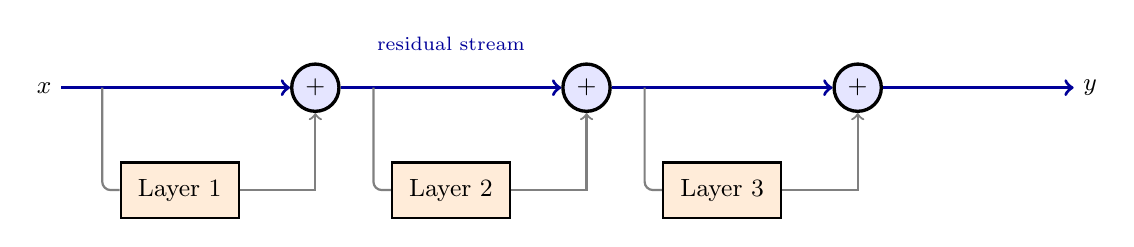
\begin{tikzpicture}[
  box/.style={rectangle, draw, thick, fill=orange!15, minimum width=1.5cm, minimum height=0.7cm, font=\small},
  stream/.style={->, very thick, blue!60!black},
  plus/.style={circle, draw, very thick, fill=blue!10, minimum size=6mm, inner sep=0pt, font=\small\bfseries},
  xscale=0.82,
]
  \node[font=\small] (x0) at (0, 0) {$x$};
  \node[plus] (p1) at (4.2, 0) {$+$};
  \node[plus] (p2) at (8.4, 0) {$+$};
  \node[plus] (p3) at (12.6, 0) {$+$};
  \node[font=\small] (xn) at (16.2, 0) {$y$};

  \draw[stream] (x0) -- (p1);
  \draw[stream] (p1) -- (p2);
  \draw[stream] (p2) -- (p3);
  \draw[stream] (p3) -- (xn);

  \node[box] (f1) at (2.1, -1.3) {Layer 1};
  \node[box] (f2) at (6.3, -1.3) {Layer 2};
  \node[box] (f3) at (10.5, -1.3) {Layer 3};

  \draw[thick, gray, rounded corners=3pt] (0.9, 0) |- (f1.west);
  \draw[->, thick, gray] (f1.east) -| (p1);
  \draw[thick, gray, rounded corners=3pt] (5.1, 0) |- (f2.west);
  \draw[->, thick, gray] (f2.east) -| (p2);
  \draw[thick, gray, rounded corners=3pt] (9.3, 0) |- (f3.west);
  \draw[->, thick, gray] (f3.east) -| (p3);

  \node[blue!60!black, font=\scriptsize, above] at (6.3, 0.35) {residual stream};
\end{tikzpicture}
\end{center}
\end{frame}

\begin{frame}{Convolutional Neural Networks}
\begin{center}
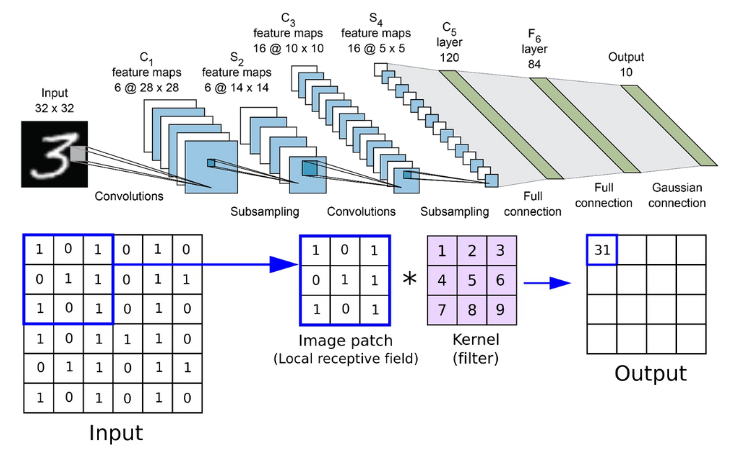
\includegraphics[width=0.95\textwidth,height=0.8\textheight,keepaspectratio]{figures/cnn_architecture.png}
\end{center}

\source{superannotate2023}
\end{frame}

\begin{frame}{Transformers}
\begin{center}
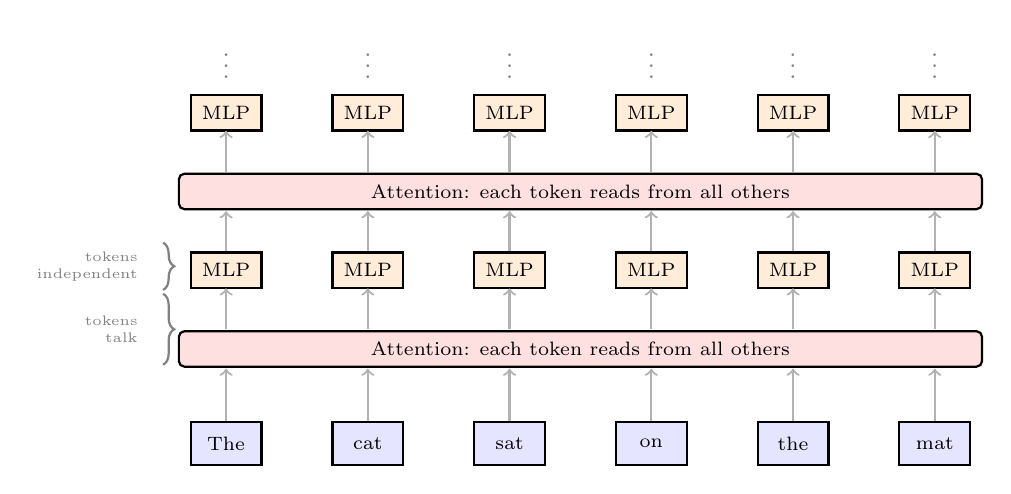
\begin{tikzpicture}[
  tok/.style={rectangle, draw, thick, fill=blue!10, minimum width=0.9cm, minimum height=0.55cm, font=\scriptsize},
  ffn/.style={rectangle, draw, thick, fill=orange!15, minimum width=0.9cm, minimum height=0.45cm, font=\scriptsize},
  attn/.style={rectangle, draw, thick, fill=red!12, rounded corners=2pt, minimum height=0.45cm, font=\scriptsize},
  arr/.style={->, thick, gray!60},
]
  \node[tok] (tA) at (0, 0) {The};
  \node[tok] (tB) at (1.8, 0) {cat};
  \node[tok] (tC) at (3.6, 0) {sat};
  \node[tok] (tD) at (5.4, 0) {on};
  \node[tok] (tE) at (7.2, 0) {the};
  \node[tok] (tF) at (9, 0) {mat};

  \node[attn, minimum width=10.2cm] (a1) at (4.5, 1.2) {Attention: each token reads from all others};

  \foreach \x in {0, 1.8, 3.6, 5.4, 7.2, 9}
    \draw[arr] (\x, 0.28) -- (\x, 0.95);

  \node[ffn] (fA1) at (0, 2.2) {MLP};
  \node[ffn] (fB1) at (1.8, 2.2) {MLP};
  \node[ffn] (fC1) at (3.6, 2.2) {MLP};
  \node[ffn] (fD1) at (5.4, 2.2) {MLP};
  \node[ffn] (fE1) at (7.2, 2.2) {MLP};
  \node[ffn] (fF1) at (9, 2.2) {MLP};

  \foreach \x in {0, 1.8, 3.6, 5.4, 7.2, 9}
    \draw[arr] (\x, 1.45) -- (\x, 1.97);

  \node[attn, minimum width=10.2cm] (a2) at (4.5, 3.2) {Attention: each token reads from all others};

  \draw[arr] (fA1.north) -- (0, 2.95);
  \draw[arr] (fB1.north) -- (1.8, 2.95);
  \draw[arr] (fC1.north) -- (3.6, 2.95);
  \draw[arr] (fD1.north) -- (5.4, 2.95);
  \draw[arr] (fE1.north) -- (7.2, 2.95);
  \draw[arr] (fF1.north) -- (9, 2.95);

  \node[ffn] (fA2) at (0, 4.2) {MLP};
  \node[ffn] (fB2) at (1.8, 4.2) {MLP};
  \node[ffn] (fC2) at (3.6, 4.2) {MLP};
  \node[ffn] (fD2) at (5.4, 4.2) {MLP};
  \node[ffn] (fE2) at (7.2, 4.2) {MLP};
  \node[ffn] (fF2) at (9, 4.2) {MLP};

  \foreach \x in {0, 1.8, 3.6, 5.4, 7.2, 9}
    \draw[arr] (\x, 3.45) -- (\x, 3.97);

  \foreach \x in {0, 1.8, 3.6, 5.4, 7.2, 9} {
    \node[gray, font=\small] at (\x, 4.9) {$\vdots$};
  }

  \draw[decorate, decoration={brace, amplitude=4pt}, thick, gray]
    (-0.8, 1.9) -- (-0.8, 1.0);
  \node[font=\tiny, gray, left, align=right] at (-1, 1.45) {tokens\\talk};

  \draw[decorate, decoration={brace, amplitude=4pt}, thick, gray]
    (-0.8, 2.55) -- (-0.8, 1.95);
  \node[font=\tiny, gray, left, align=right] at (-1, 2.25) {tokens\\independent};
\end{tikzpicture}
\end{center}
\end{frame}

\begin{frame}{Attention}
\vspace{-0.3em}
\begin{center}
\begin{tikzpicture}[
  mat/.style={rectangle, draw, thick, minimum width=1.3cm, minimum height=0.6cm, font=\normalsize\bfseries},
  wt/.style={rectangle, draw, thick, dashed, fill=gray!6, minimum width=1.1cm, minimum height=0.5cm, font=\small},
  op/.style={rectangle, draw, thick, rounded corners=3pt, fill=gray!8, minimum height=0.5cm, font=\small},
  sh/.style={font=\small, text=gray!80},
  arr/.style={->, thick, gray!55},
  scale=0.88, transform shape,
]
  % Row 1: Input X
  \node[mat, fill=green!15, minimum width=1.6cm] (X) at (1.5, 0) {$X$};
  \node[sh, right=0.15cm of X] {$n \times d$};

  % Row 2: Learned projection weights (dashed = learned parameters)
  \node[wt, fill=red!8] (Wq) at (-2, 1.2) {$W_Q$};
  \node[sh, right=0.1cm of Wq] {$d \!\times\! d_h$};
  \node[wt, fill=blue!8] (Wk) at (1.5, 1.2) {$W_K$};
  \node[sh, right=0.1cm of Wk] {$d \!\times\! d_h$};
  \node[wt, fill=orange!8] (Wv) at (5, 1.2) {$W_V$};
  \node[sh, right=0.1cm of Wv] {$d \!\times\! d_h$};

  \draw[arr] (X.north) -- ++(0,0.1) -| (Wq.south);
  \draw[arr] (X.north) -- (Wk.south);
  \draw[arr] (X.north) -- ++(0,0.1) -| (Wv.south);

  % Row 3: Q K V
  \node[mat, fill=red!20] (Q) at (-2, 2.3) {$Q$};
  \node[sh, right=0.15cm of Q] {$n \times d_h$};
  \node[mat, fill=blue!20] (K) at (1.5, 2.3) {$K$};
  \node[sh, right=0.15cm of K] {$n \times d_h$};
  \node[mat, fill=orange!25] (V) at (5, 2.3) {$V$};
  \node[sh, right=0.15cm of V] {$n \times d_h$};

  \draw[arr] (Wq.north) -- (Q.south);
  \draw[arr] (Wk.north) -- (K.south);
  \draw[arr] (Wv.north) -- (V.south);

  % Row 4: QK^T / sqrt(d)
  \node[op, fill=yellow!15] (qkt) at (-0.25, 3.5) {$QK^\top\! / \sqrt{d_h}$};
  \node[sh, right=0.15cm of qkt] {$n \times n$};
  \draw[arr] (Q.north) -- ++(0,0.2) -| ($(qkt.south)+(-0.5,0)$);
  \draw[arr] (K.north) -- ++(0,0.2) -| ($(qkt.south)+(0.5,0)$);

  % Row 5: softmax → A (softmax as label on arrow)
  \node[mat, fill=purple!18, minimum width=1cm, minimum height=0.55cm, font=\small\bfseries] (A) at (-0.25, 4.7) {$A$};
  \node[sh, right=0.15cm of A] {$n \times n$};
  \draw[arr] (qkt.north) -- node[left, font=\small, text=gray!65, inner sep=2pt] {softmax} (A.south);

  % Row 6: A * V → output
  \node[mat, fill=green!18, minimum width=1.5cm] (av) at (2.5, 5.8) {$A \cdot V$};
  \node[sh, right=0.15cm of av] {$n \times d_h$};
  \draw[arr] (A.north) -- ++(0,0.15) -| ($(av.south)+(-0.4,0)$);
  \draw[arr] (V.north) -- ++(0,2.55) -| ($(av.south)+(0.4,0)$);

  % Equation
  \node[font=\large, align=left] at (9, 3.3) {
    $\text{Attention}(Q,K,V)$\\[0.8em]
    $= \text{softmax}\!\left(\dfrac{QK^\top}{\sqrt{d_h}}\right) V$
  };

  % Legend
  \node[align=left, font=\normalsize, text=gray!80] at (9, 0.6) {
    $n$ = sequence length\\[0.3em]
    $d$ = model dimension\\[0.3em]
    $d_h$ = head dimension
  };
\end{tikzpicture}
\end{center}
\end{frame}

% ============================================================
\section{Mechanistic Interpretability}
% ============================================================

% ------------------------------------------------------------
\subsection{What is Mechanistic Interpretability?}
% ------------------------------------------------------------

\begin{frame}{}
\begin{enumerate}
\item Machine Learning
  \begin{enumerate}
  \item[1.1] Concepts
  \item[1.2] Architectures
  \end{enumerate}
\item \textbf{\large Mechanistic Interpretability}
  \begin{enumerate}
  \item[2.1] \textbf{What is Mechanistic Interpretability?} $\leftarrow$
  \end{enumerate}
\item \textcolor{gray}{Features}
\item \textcolor{gray}{Circuits}
\item \textcolor{gray}{Open Problems}
\end{enumerate}
\end{frame}

\begin{frame}{Two Ways to Relate to Models}
\begin{columns}[T]
\begin{column}{0.48\textwidth}
\begin{center}
\textbf{\large Machine Learning}
\vspace{0.5em}

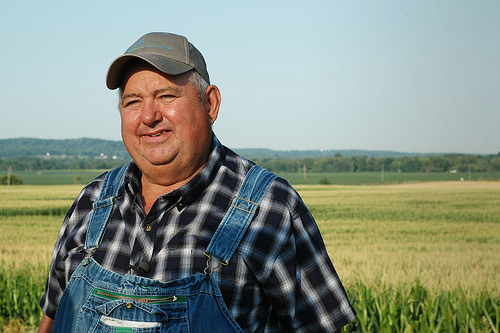
\includegraphics[width=0.75\textwidth]{figures/honest_work.jpg}
\end{center}

\begin{itemize}
\item Output-oriented
\item Find hyperparameters to improve models
\end{itemize}
\end{column}

\begin{column}{0.48\textwidth}
\begin{center}
\textbf{\large Mech.\ Interpretability}
\vspace{0.5em}

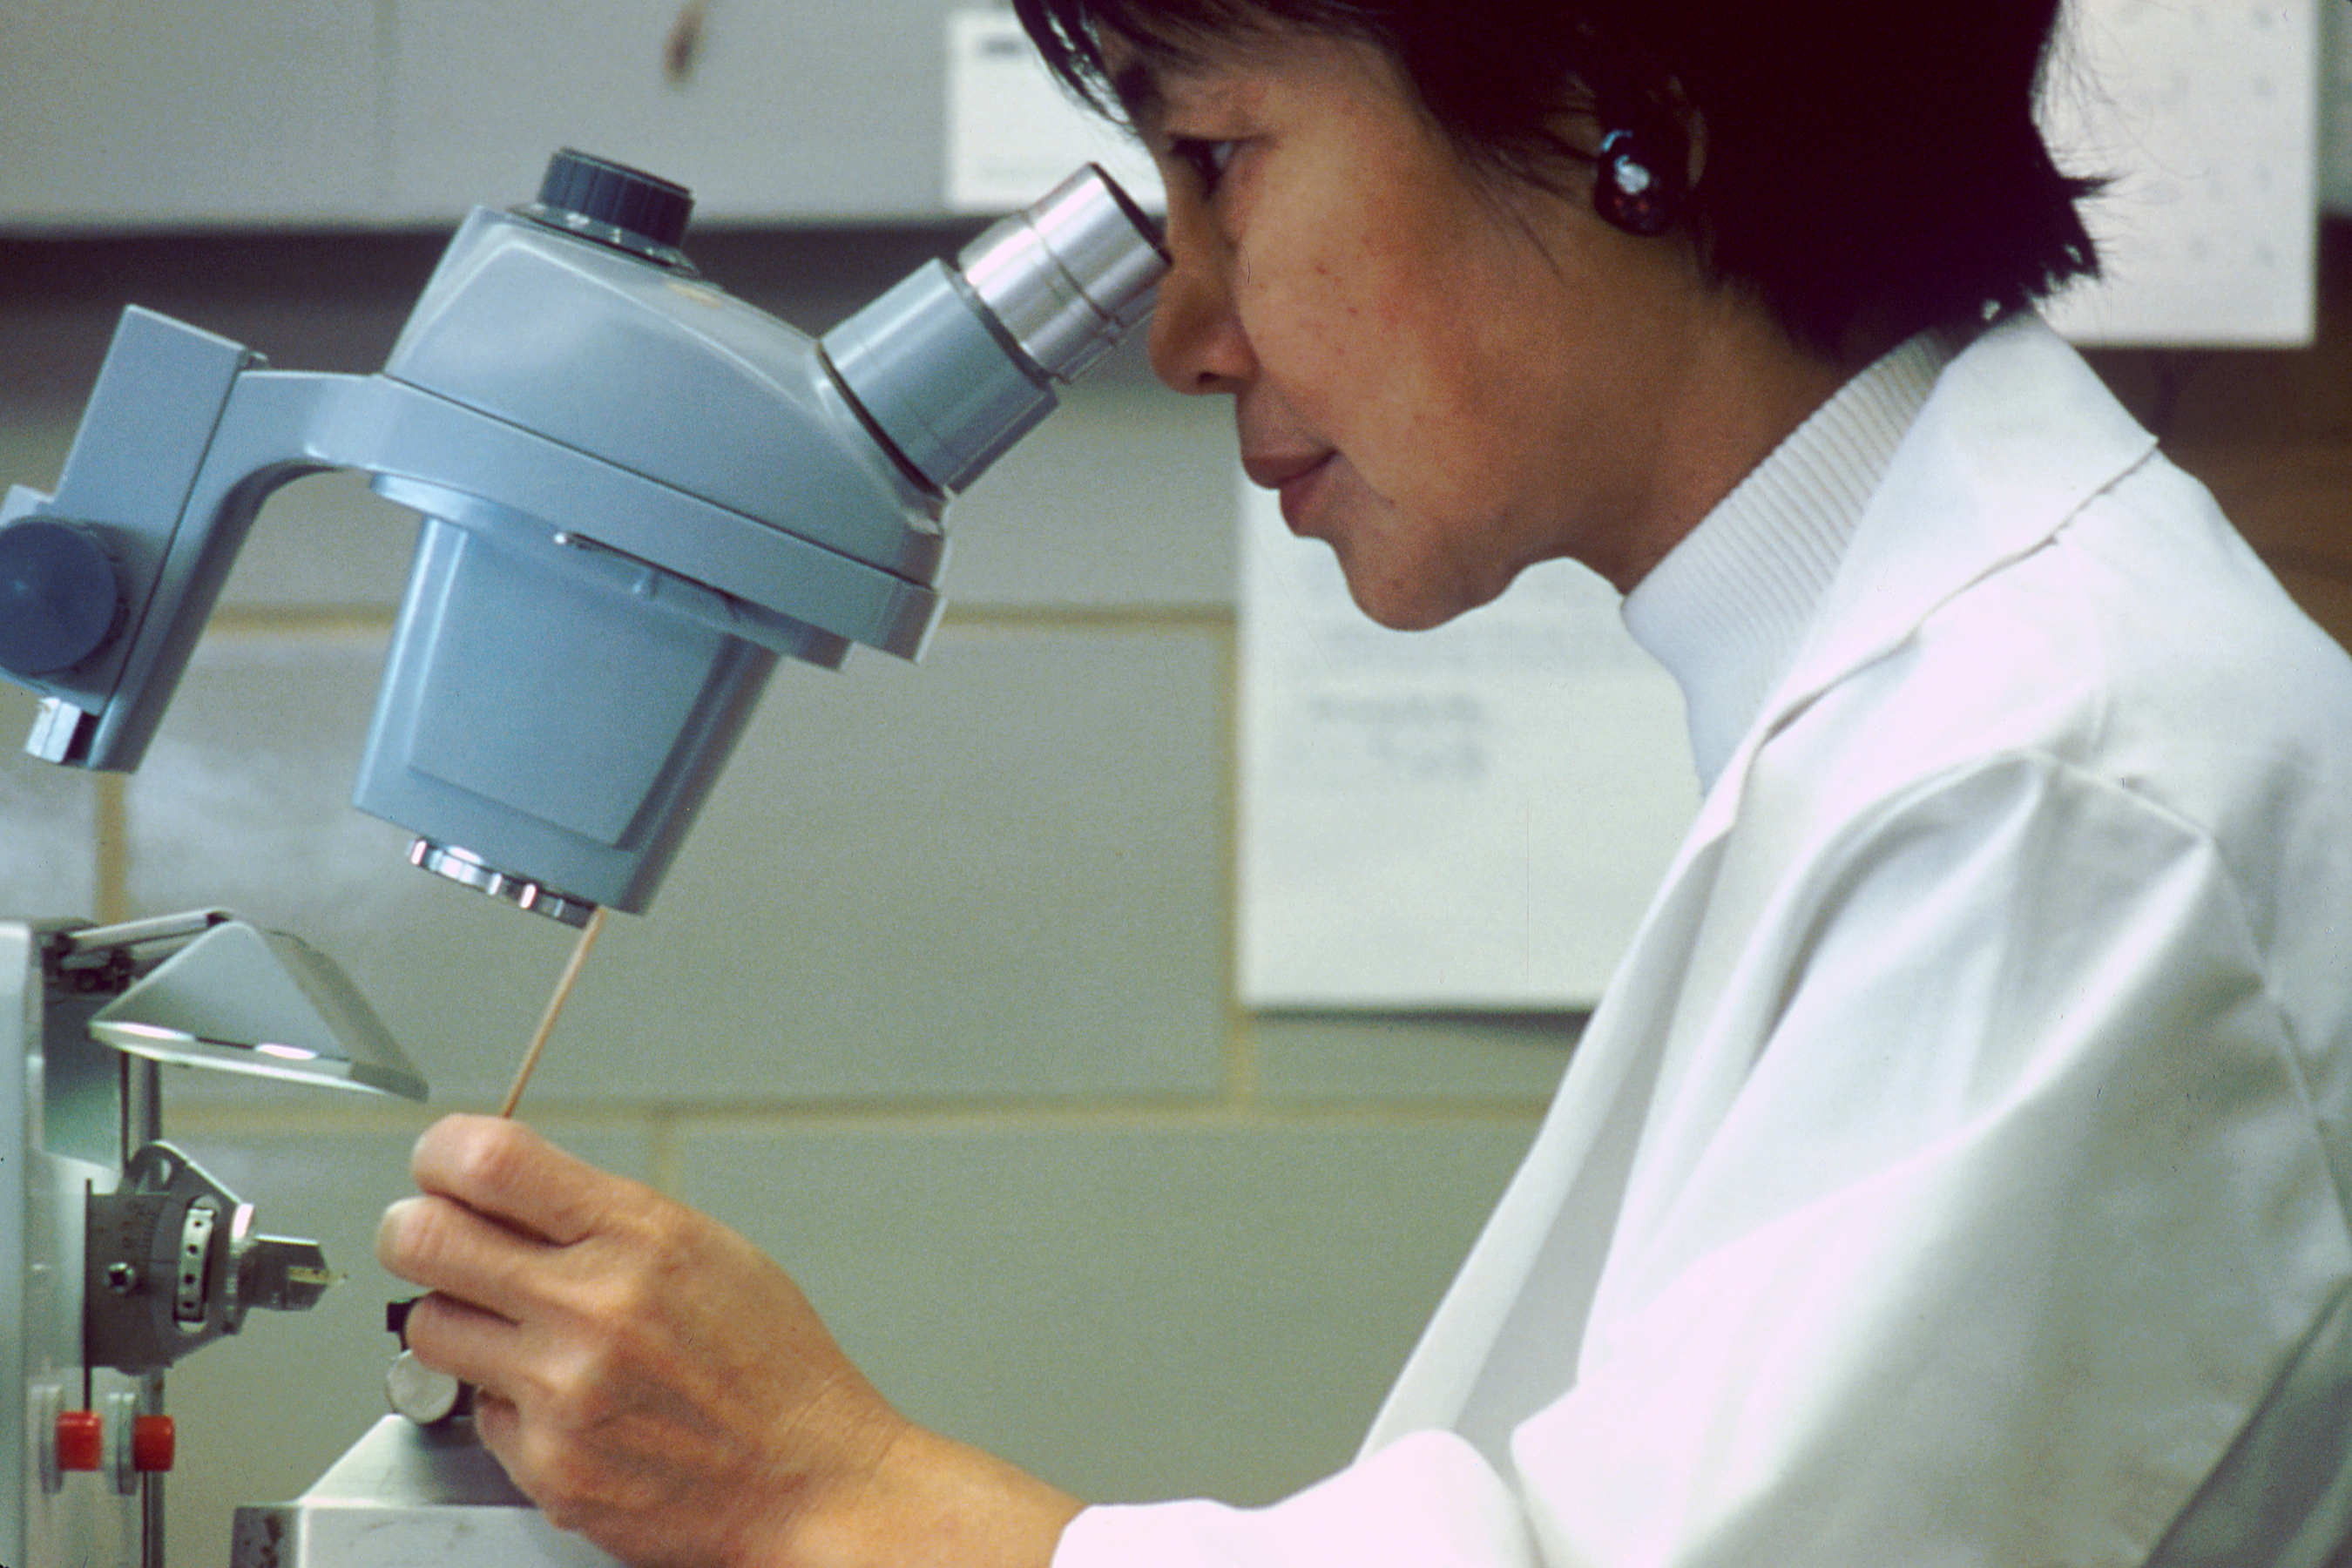
\includegraphics[width=0.75\textwidth]{figures/scientist_microscope.jpg}
\end{center}

\begin{itemize}
\item Learned models are the object of study
\item Understand and reverse-engineer parameters
\end{itemize}
\end{column}
\end{columns}
\end{frame}

\begin{frame}{Theories of Impact}
\vfill
\begin{center}
\begin{minipage}{0.7\textwidth}
\Large
\begin{itemize}
\item Auditing for misalignment/deception
\item Enumerative safety
\item Eliciting latent knowledge
\end{itemize}
\end{minipage}
\end{center}
\vfill

\source{nanda2022}
\end{frame}

\begin{frame}{Three Speculative Claims}
\begin{enumerate}
\item \textbf{Features} are the fundamental unit of neural networks.
They correspond to directions.
These features can be rigorously studied and understood.

\vspace{0.5em}
\item Features are connected by weights, forming \textbf{circuits}.
These circuits can also be rigorously studied and understood.

\vspace{0.5em}
\item \textbf{Universality}: Analogous features and circuits form across models and tasks.
\end{enumerate}

\source{olah2020}
\end{frame}

% ------------------------------------------------------------
\subsection{MechInterp in CNNs}
% ------------------------------------------------------------

\begin{frame}{}
\begin{enumerate}
\item Machine Learning
  \begin{enumerate}
  \item[1.1] Concepts
  \item[1.2] Architectures
  \end{enumerate}
\item \textbf{\large Mechanistic Interpretability}
  \begin{enumerate}
  \item[2.1] What is Mechanistic Interpretability?
  \item[2.2] \textbf{MechInterp in CNNs} $\leftarrow$
  \end{enumerate}
\item \textcolor{gray}{Features}
\item \textcolor{gray}{Circuits}
\item \textcolor{gray}{Open Problems}
\end{enumerate}
\end{frame}

\begin{frame}{Convolutional Neural Networks}
\begin{center}
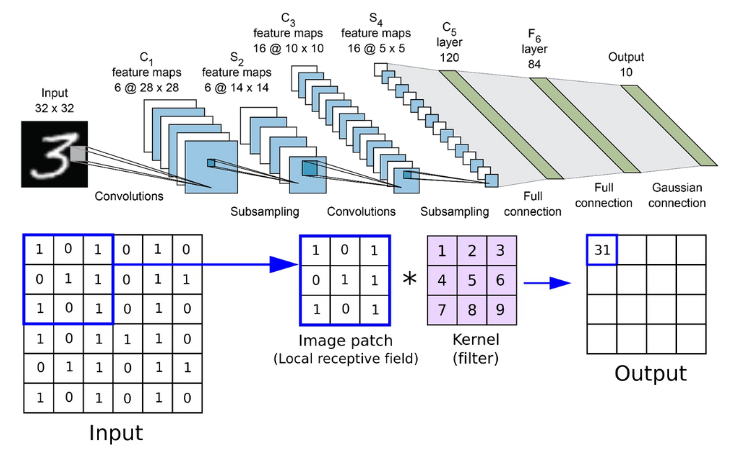
\includegraphics[width=0.95\textwidth,height=0.8\textheight,keepaspectratio]{figures/cnn_architecture.png}
\end{center}

\source{superannotate2023}
\end{frame}

\begin{frame}{Evidence for Curve Detectors}
\begin{center}
\begin{tikzpicture}[
  img/.style={rectangle, draw=gray!50, thick, inner sep=2pt},
  lbl/.style={font=\scriptsize, align=center},
]
  \node[img] (fv) at (0, 0) {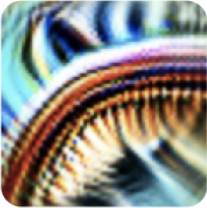
\includegraphics[width=2.8cm]{figures/curve_detector_feature_visualization.png}};
  \node[lbl, below=2pt of fv] {Feature\\Visualization};

  \node[img] (de) at (4, 0) {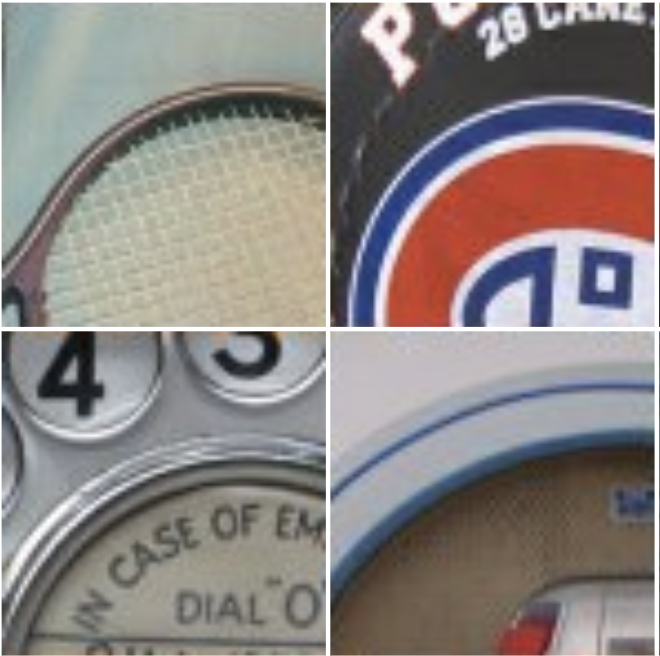
\includegraphics[width=2.8cm]{figures/curve_detector_dataset_examples.png}};
  \node[lbl, below=2pt of de] {Dataset\\Examples};

  \node[img] (st) at (8, 0) {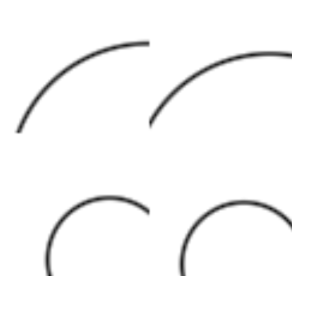
\includegraphics[width=2.8cm]{figures/curve_detector_synthetic_tuning.png}};
  \node[lbl, below=2pt of st] {Synthetic\\Tuning};

  \node[img] (rt) at (0, -3.8) {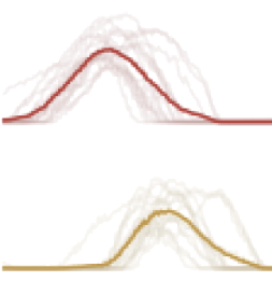
\includegraphics[width=2.8cm]{figures/curve_detector_radial_tuning.png}};
  \node[lbl, below=2pt of rt] {Joint\\Tuning};

  \node[img] (wt) at (4, -3.8) {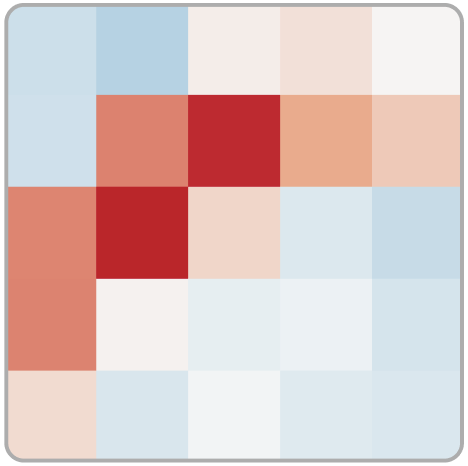
\includegraphics[width=2.8cm]{figures/curve_detector_weights.png}};
  \node[lbl, below=2pt of wt] {Weight\\Analysis};

  \node[img] (uc) at (8, -3.8) {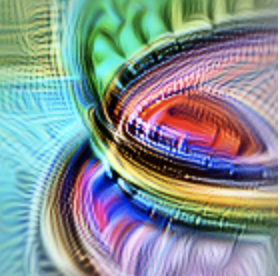
\includegraphics[width=2.8cm]{figures/curve_detector_use_in_circuits.png}};
  \node[lbl, below=2pt of uc] {Use in\\Circuits};
\end{tikzpicture}
\end{center}

\source{olah2020}
\end{frame}

\begin{frame}{Circuits: Car Detection}
\begin{center}
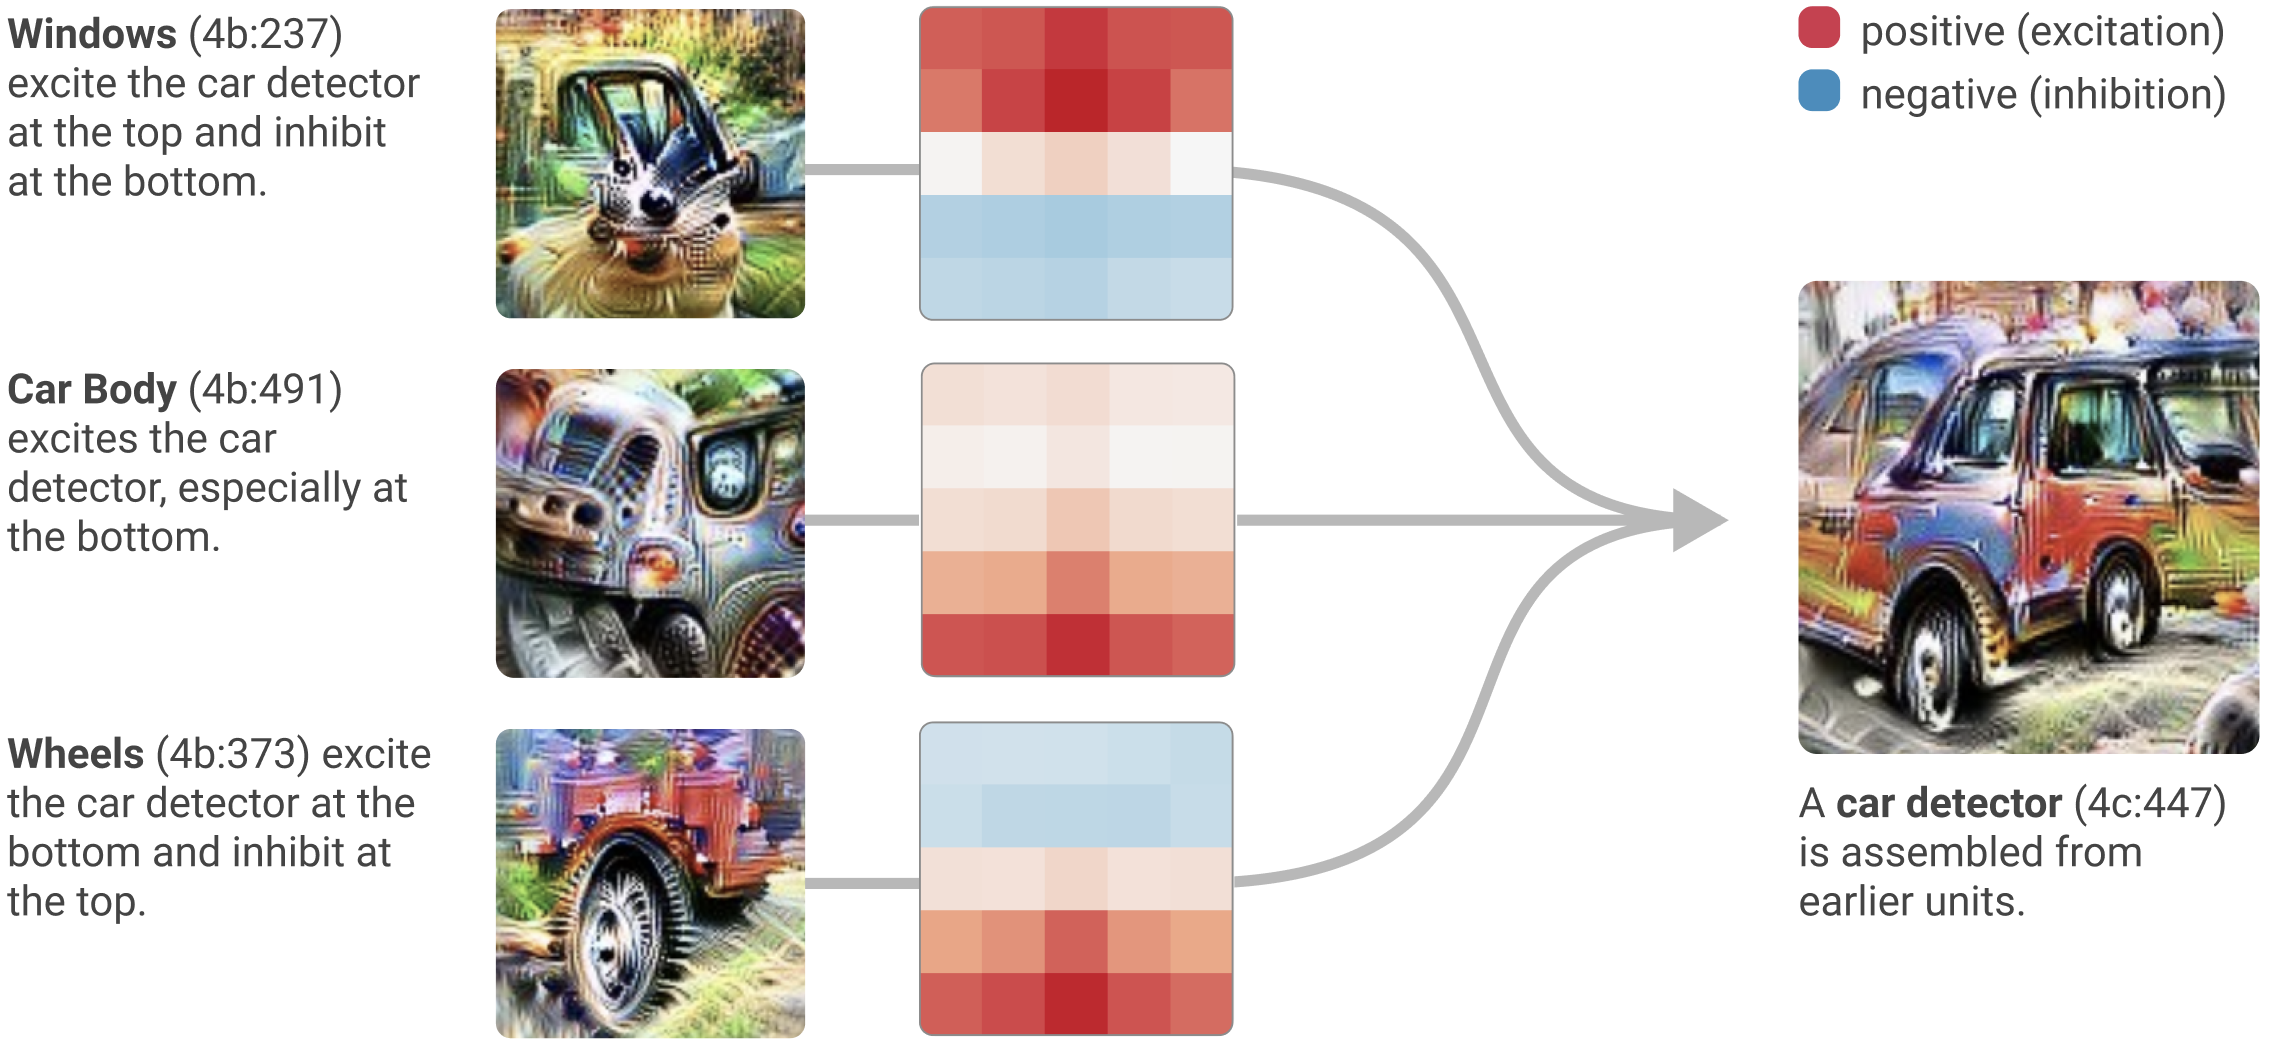
\includegraphics[width=0.85\textwidth,height=0.75\textheight,keepaspectratio]{figures/car_circuit.png}
\end{center}

\source{olah2020}
\end{frame}

\begin{frame}{Universality in Image Models}
\begin{center}
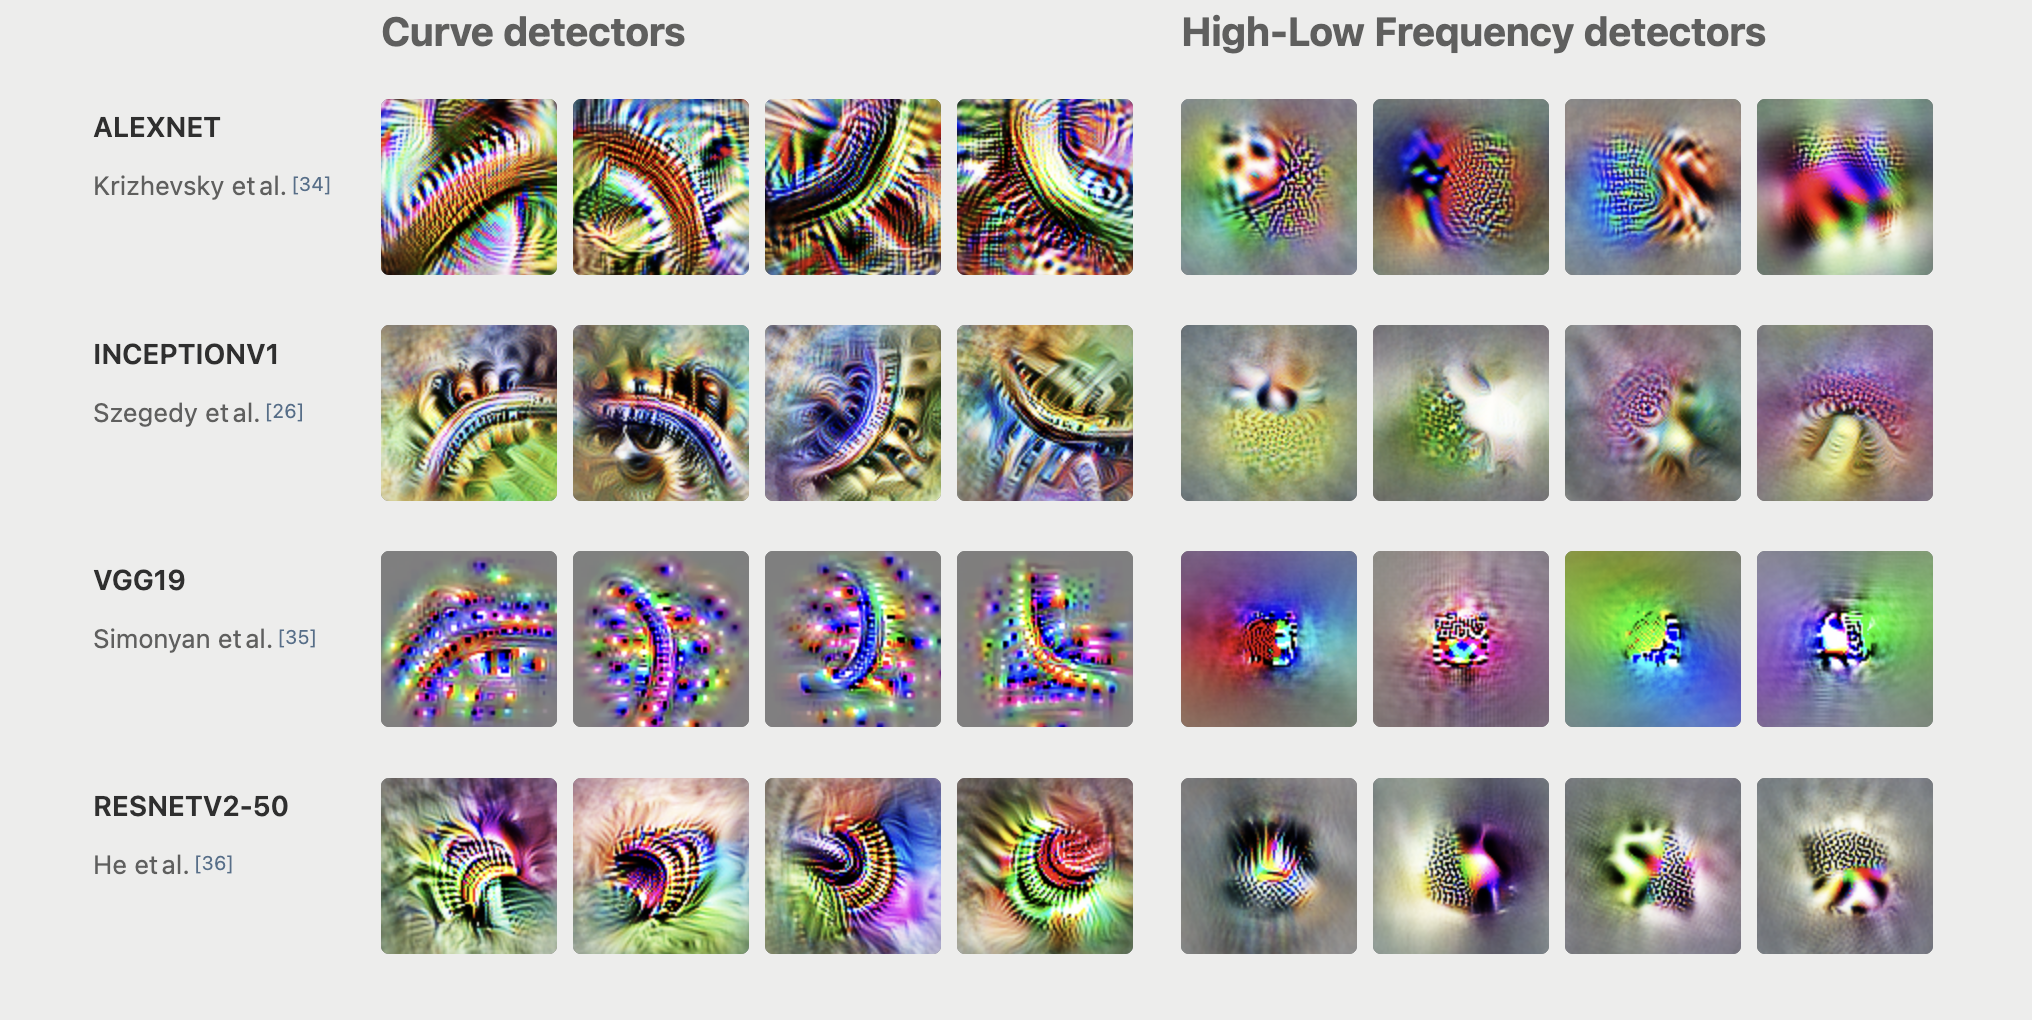
\includegraphics[width=0.95\textwidth,height=0.8\textheight,keepaspectratio]{figures/universality.png}
\end{center}

\source{olah2020}
\end{frame}

% ============================================================
\section{Features in Transformers}
% ============================================================

\begin{frame}{}
\begin{enumerate}
\item Machine Learning
  \begin{enumerate}
  \item[1.1] Concepts
  \item[1.2] Architectures
  \end{enumerate}
\item Mechanistic Interpretability
  \begin{enumerate}
  \item[2.1] What is Mechanistic Interpretability?
  \item[2.2] MechInterp in CNNs
  \end{enumerate}
\item \textbf{\large Features in Transformers} $\leftarrow$
\item \textcolor{gray}{Circuits}
\item \textcolor{gray}{Open Problems}
\end{enumerate}
\end{frame}

\begin{frame}{Getting a Feature Direction}
\textbf{Contrastive pairs:}
\[ r = \text{Emb}(\text{``Spanish''}) - \text{Emb}(\text{``French''}) \]

\vspace{0.5em}
\textbf{Linear probe:} \quad {\small $x_i$: sample activation, $y_i \in \{+1, -1\}$: label}
\[ r = \arg\max_{\|r\|=1} \sum_i y_i \cdot r^\top x_i \]

\vspace{0.5em}
\textbf{CAA:} \quad {\small $x_i^{(+)}, x_i^{(-)}$: positive/negative example of a property}
\[ r = \frac{1}{N} \sum_{i=1}^{N} \left( x_i^{(+)} - x_i^{(-)} \right) \]
\end{frame}

\begin{frame}{What To Do with a Feature Direction}
\textbf{Activation addition} (steering):
\[ x' \leftarrow x + \alpha \cdot r \]

\vspace{0.5em}
\textbf{Direction ablation} (make the model blind to the concept):
\[ x' \leftarrow x - \hat{r}\hat{r}^\top x \]

\vspace{0.5em}
\textbf{Probing} (read out a concept):
\[ s = r^\top x \]

\vspace{0.3em}
{\small $r$: feature direction \quad $x$: activation \quad $\alpha$: steering strength}

\source{arditi2024}
\end{frame}

\begin{frame}{Example: Language Direction}
\paperfig{figures/park2024/fig3.png}{06_edinburgh/figures/park2024/fig3-caption.txt}

\source{park2024}
\end{frame}

\begin{frame}{Example: Probing for Truthfulness}
\paperfig{figures/li2024b/fig1.png}{06_edinburgh/figures/li2024b/fig1-caption.txt}

\source{li2024b}
\end{frame}

\begin{frame}{Example: Inference-Time Intervention}
\paperfig{figures/li2024b/fig2.png}{06_edinburgh/figures/li2024b/fig2-caption.txt}

\source{li2024b}
\end{frame}

\begin{frame}{Example: ITI Improves Truthfulness}
\paperfig{figures/li2024b/table0.png}{06_edinburgh/figures/li2024b/table0-caption.txt}

\source{li2024b}
\end{frame}

\begin{frame}{Example: Contrastive Activation Addition}
\paperfig{figures/panickssery2024/fig0.png}{06_edinburgh/figures/panickssery2024/fig0-caption.txt}

\source{panickssery2024}
\end{frame}

\begin{frame}{Example: CAA Steers Arbitrary Behaviors}
\paperfig{figures/panickssery2024/fig7.png}{06_edinburgh/figures/panickssery2024/fig7-caption.txt}

\source{panickssery2024}
\end{frame}

\begin{frame}{Example: Othello-GPT World Model}
\paperfig{figures/nanda2023/fig0.png}{06_edinburgh/figures/nanda2023/fig0-caption.txt}

\source{nanda2023}
\end{frame}

\begin{frame}{Example: Intervening on the World Model}
\paperfig{figures/nanda2023/fig1.png}{06_edinburgh/figures/nanda2023/fig1-caption.txt}

\source{nanda2023}
\end{frame}

\begin{frame}{Example: Refusal Is a Single Direction}
\paperfig{figures/arditi2024/fig0.png}{06_edinburgh/figures/arditi2024/fig0-caption.txt}

\source{arditi2024}
\end{frame}

\begin{frame}{Example: Adding Refusal to Harmless Queries}
\paperfig{figures/arditi2024/fig1.png}{06_edinburgh/figures/arditi2024/fig1-caption.txt}

\source{arditi2024}
\end{frame}
